\begin{flushright} {\tiny {\color{gray} learning\_python.tex}} \end{flushright}
%~~~~~~~~~~~~~~~~~~~~~~~~~~~~~~~~~~~~~~~~~~~~~~~~~~~~~~~~~~~~~~~~~~~~~~~~~~~~~~

\begin{itemize}
\item Introduction to Python \& Data (Utrecht University)\\
\url{https://utrechtuniversity.github.io/workshop-introduction-to-python/}

\item 
This is a joint course for geography and geology students at the Department of 
Geosciences and Geography, University of Helsinki\\
\url{https://geo-python.github.io/site/}

\item Python for Earth Science Students (University of California San Diego)\\
\url{https://github.com/ltauxe/Python-for-Earth-Science-Students}

\item \url{https://www.w3schools.com/python/default.asp}

\item \url{https://www.codecademy.com/learn/learn-python}

\item \url{https://learnpythonthehardway.org/book/}

\item \url{https://software-carpentry.org/lessons/} core lessons:
\begin{itemize}
\item The Unix Shell
\item Version Control with Git
\item Programming with Python
\item Plotting and Programming in Python
\item Programming with R
\item R for Reproducible Scientific Analysis
\end{itemize}


\end{itemize}

%--------------------------
\subsection{Sparse matrices}

So far, the best way I have found to deal with sparse matrices is to 
declare the matrix as a 'lil\_matrix' (linked list).

\begin{lstlisting}
from scipy.sparse import csr_matrix, lil_matrix
A_mat = lil_matrix((Nfem,Nfem),dtype=np.float64)
\end{lstlisting}

One then adds terms to it as if it was a full/dense matrix. 
Once the assembly is done, the conversion to CSR format is trivial:

\begin{lstlisting}
A_mat=A_mat.tocsr()
\end{lstlisting}

Finally the solver can be called:

\begin{lstlisting}
sol=sps.linalg.spsolve(A_mat,rhs)
\end{lstlisting}

%--------------------------
\subsection{condition number}

if the matrix has been declared as lil\_matrix, first convert it to a dense matrix:
\begin{lstlisting}
A_mat=A_mat.dense()
\end{lstlisting}
The condition number of the matrix is simply obtained as follows:
\begin{lstlisting}
from numpy import linalg as LA
print(LA.cond(A_mat))
\end{lstlisting}

%--------------------------
\subsection{Weird stuff}

Python is touted as the one language students should learn 
and master. However it is a language which allows *way* too 
much liberty in its syntax and encourages students to be sloppy. 

For instance the following code runs just fine:

\begin{lstlisting}
for k in range(0,5): 
    for k in range(0,5):
        for k in range(0,5):
            print (k)
\end{lstlisting}

This alone should disqualify this language. It is easy to see the obvious problem with this code, but adding a few lines of code in between each 'for' line hides the problem and the absence of any warning makes this code a nightmare to debug.

Here is another example:

\begin{lstlisting}
import numpy as np

Told=np.full(10,123)

Tnew=np.zeros(10)
for i in range(0,10):
    Tnew[i]=np.sqrt(i**5)

print(Tnew)

Told[:]=Tnew[:]

print(Told)
\end{lstlisting}
If Told is not defined explicitely as a float, then the 
numer 123 will decide of its type (in this case 
integer). If `123' is changed into `123.' then the 
array will be initialised as an array of floats.
In the first case 
\begin{verbatim}
Told is [  0   1   5  15  32  55  88 129 181 243]
\end{verbatim}
while in the second case it is equal to 
\begin{verbatim}
[  0.           1.           5.65685425  15.58845727  32.
  55.90169944  88.18163074 129.64181424 181.01933598 243.        ] 
\end{verbatim}
This is very dangerous since our students are not taught 
number representation.

\begin{verbatim}
https://www.w3schools.com/python/default.asp

https://www.codecademy.com/learn/learn-python

https://learnpythonthehardway.org/book/
\end{verbatim}

%----------------------------------
\subsection{Making simple 2D plots}

\begin{lstlisting}
import matplotlib.pyplot as plt

# number of points
N=100

# a despicable way of filling two arrays
x_data=[]
y_data=[]
for i in range(0,N):
    x=i
    y=i**2+2*i+1.
    x_data.append(x)
    y_data.append(y)

# generating a 2D figure with the data
plt.figure()
plt.plot(x_data,y_data, label = 'name of data')
plt.xlabel('x-axis label')
plt.ylabel('y-axis label')
plt.legend()
plt.savefig('myplot.pdf', bbox_inches='tight')
plt.show()
\end{lstlisting}

\begin{center}
\includegraphics[width=7cm]{images/python/myplot}
\end{center}



%----------------------------------
\subsection{Making simple 3D plots of scatter}

\begin{lstlisting}
fig = plt.figure()
ax = plt.axes(projection='3d')
ax.set_title("insert here text for title")
size = ..some value..
ax.scatter3D(x, y, z, s = size)
\end{lstlisting}




%----------------------------------
\subsection{How to debug your code}


Debugging a FE code is by no means trivial. There is (at least) a grid, a connectivity array, basis functions and their derivatives, the elemental matrices and rhs, the assembly, boundary conditions, and a call to a solver before the solution (if the solver returns one!) can be visualised. 
\begin{itemize}
\item First and foremost, make sure that your grid of points is correct.
For instance, you can resort to exporting it to an ascii file as follows:
\begin{lstlisting}
np.savetxt('velocity.ascii',np.array([x,y,u,v]).T,header='# x,y,u,v')
\end{lstlisting}
In two dimensions, you should set for example nelx=3 and nely=2, so that 
for $Q_1$ elements the grid counts 12 points. Then make sure the coordinates and the order of the points makes sense. 
Repeat the process for pressure nodes, temperature nodes, etc ...

\item Then it is time to check the connectivity array(s). 
\begin{lstlisting}
for iel in range (0,nel):
   print ("iel=",iel)
   for k in range(0,m)
      print ("node ",icon[0,iel],"at pos.",x[icon[0,iel]], y[icon[0,iel]])
\end{lstlisting}
This displays the list of nodes and their positions making each element.
Repeat the process for every connectivity array.

\item We can go on with testing that the all basis functions are 1 on their node and  zero elsewhere:
\begin{lstlisting}
for i in range(0,m):
   print ('node',i,':',NNV(rnodes[i],snodes[i]))
\end{lstlisting}
here the arrays rnodes and snodes contain the (r,s) coordinates of the m nodes 

\item test jacobian, compute volume of domain

\item sum(dNNNdx)=0

\item print nodes where bc 

\end{itemize}

%----------------------------------
\subsection{Optional arguments}

Courtesy of Henry Brett.

\begin{lstlisting}
def myfunc(a,b, *optional_arguments, **keyword_arguments):
    print(a)
    print(b)
    for ar in optional_arguments:
        print(ar)
    d=keyword_arguments.get("d", None)
    print(d)
    

a="dog"
b="cat"
myfunc(a,b,"shrek","fiona",d="donkey")
\end{lstlisting}

%------------------------------------------------
\subsection{drawing and filling quadrilaterals}

\begin{lstlisting}
import matplotlib.pyplot as plt

plt.figure(figsize=(3, 3))
plt.axis('equal')

x=(1,1.5,1.6,0.8)
y=(0,-0.1,1.5,1.2)
plt.fill(x, y,"b")

x=(0,0.5,0.6,-0.2)
y=(0,-0.4,1.1,1.1)
plt.fill(x, y,"r")

plt.savefig('xxx.pdf')
plt.show()

\end{lstlisting}

\begin{center}
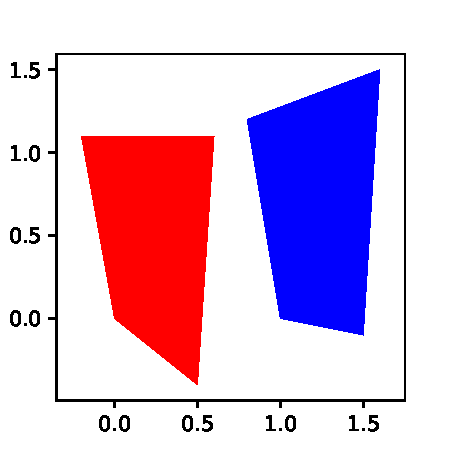
\includegraphics[width=5cm]{images/python/xxx}
\end{center}

